\documentclass[1p]{elsarticle_modified}
%\bibliographystyle{elsarticle-num}

%\usepackage[colorlinks]{hyperref}
%\usepackage{abbrmath_seonhwa} %\Abb, \Ascr, \Acal ,\Abf, \Afrak
\usepackage{amsfonts}
\usepackage{amssymb}
\usepackage{amsmath}
\usepackage{amsthm}
\usepackage{scalefnt}
\usepackage{amsbsy}
\usepackage{kotex}
\usepackage{caption}
\usepackage{subfig}
\usepackage{color}
\usepackage{graphicx}
\usepackage{xcolor} %% white, black, red, green, blue, cyan, magenta, yellow
\usepackage{float}
\usepackage{setspace}
\usepackage{hyperref}

\usepackage{tikz}
\usetikzlibrary{arrows}

\usepackage{multirow}
\usepackage{array} % fixed length table
\usepackage{hhline}

%%%%%%%%%%%%%%%%%%%%%
\makeatletter
\renewcommand*\env@matrix[1][\arraystretch]{%
	\edef\arraystretch{#1}%
	\hskip -\arraycolsep
	\let\@ifnextchar\new@ifnextchar
	\array{*\c@MaxMatrixCols c}}
\makeatother %https://tex.stackexchange.com/questions/14071/how-can-i-increase-the-line-spacing-in-a-matrix
%%%%%%%%%%%%%%%

\usepackage[normalem]{ulem}

\newcommand{\msout}[1]{\ifmmode\text{\sout{\ensuremath{#1}}}\else\sout{#1}\fi}
%SOURCE: \msout is \stkout macro in https://tex.stackexchange.com/questions/20609/strikeout-in-math-mode

\newcommand{\cancel}[1]{
	\ifmmode
	{\color{red}\msout{#1}}
	\else
	{\color{red}\sout{#1}}
	\fi
}

\newcommand{\add}[1]{
	{\color{blue}\uwave{#1}}
}

\newcommand{\replace}[2]{
	\ifmmode
	{\color{red}\msout{#1}}{\color{blue}\uwave{#2}}
	\else
	{\color{red}\sout{#1}}{\color{blue}\uwave{#2}}
	\fi
}

\newcommand{\Sol}{\mathcal{S}} %segment
\newcommand{\D}{D} %diagram
\newcommand{\A}{\mathcal{A}} %arc


%%%%%%%%%%%%%%%%%%%%%%%%%%%%%5 test

\def\sl{\operatorname{\textup{SL}}(2,\Cbb)}
\def\psl{\operatorname{\textup{PSL}}(2,\Cbb)}
\def\quan{\mkern 1mu \triangleright \mkern 1mu}

\theoremstyle{definition}
\newtheorem{thm}{Theorem}[section]
\newtheorem{prop}[thm]{Proposition}
\newtheorem{lem}[thm]{Lemma}
\newtheorem{ques}[thm]{Question}
\newtheorem{cor}[thm]{Corollary}
\newtheorem{defn}[thm]{Definition}
\newtheorem{exam}[thm]{Example}
\newtheorem{rmk}[thm]{Remark}
\newtheorem{alg}[thm]{Algorithm}

\newcommand{\I}{\sqrt{-1}}
\begin{document}

%\begin{frontmatter}
%
%\title{Boundary parabolic representations of knots up to 8 crossings}
%
%%% Group authors per affiliation:
%\author{Yunhi Cho} 
%\address{Department of Mathematics, University of Seoul, Seoul, Korea}
%\ead{yhcho@uos.ac.kr}
%
%
%\author{Seonhwa Kim} %\fnref{s_kim}}
%\address{Center for Geometry and Physics, Institute for Basic Science, Pohang, 37673, Korea}
%\ead{ryeona17@ibs.re.kr}
%
%\author{Hyuk Kim}
%\address{Department of Mathematical Sciences, Seoul National University, Seoul 08826, Korea}
%\ead{hyukkim@snu.ac.kr}
%
%\author{Seokbeom Yoon}
%\address{Department of Mathematical Sciences, Seoul National University, Seoul, 08826,  Korea}
%\ead{sbyoon15@snu.ac.kr}
%
%\begin{abstract}
%We find all boundary parabolic representation of knots up to 8 crossings.
%
%\end{abstract}
%\begin{keyword}
%    \MSC[2010] 57M25 
%\end{keyword}
%
%\end{frontmatter}

%\linenumbers
%\tableofcontents
%
\newcommand\colored[1]{\textcolor{white}{\rule[-0.35ex]{0.8em}{1.4ex}}\kern-0.8em\color{red} #1}%
%\newcommand\colored[1]{\textcolor{white}{ #1}\kern-2.17ex	\textcolor{white}{ #1}\kern-1.81ex	\textcolor{white}{ #1}\kern-2.15ex\color{red}#1	}

{\Large $\underline{12a_{0243}~(K12a_{0243})}$}

\setlength{\tabcolsep}{10pt}
\renewcommand{\arraystretch}{1.6}
\vspace{1cm}\begin{tabular}{m{100pt}>{\centering\arraybackslash}m{274pt}}
\multirow{5}{120pt}{
	\centering
	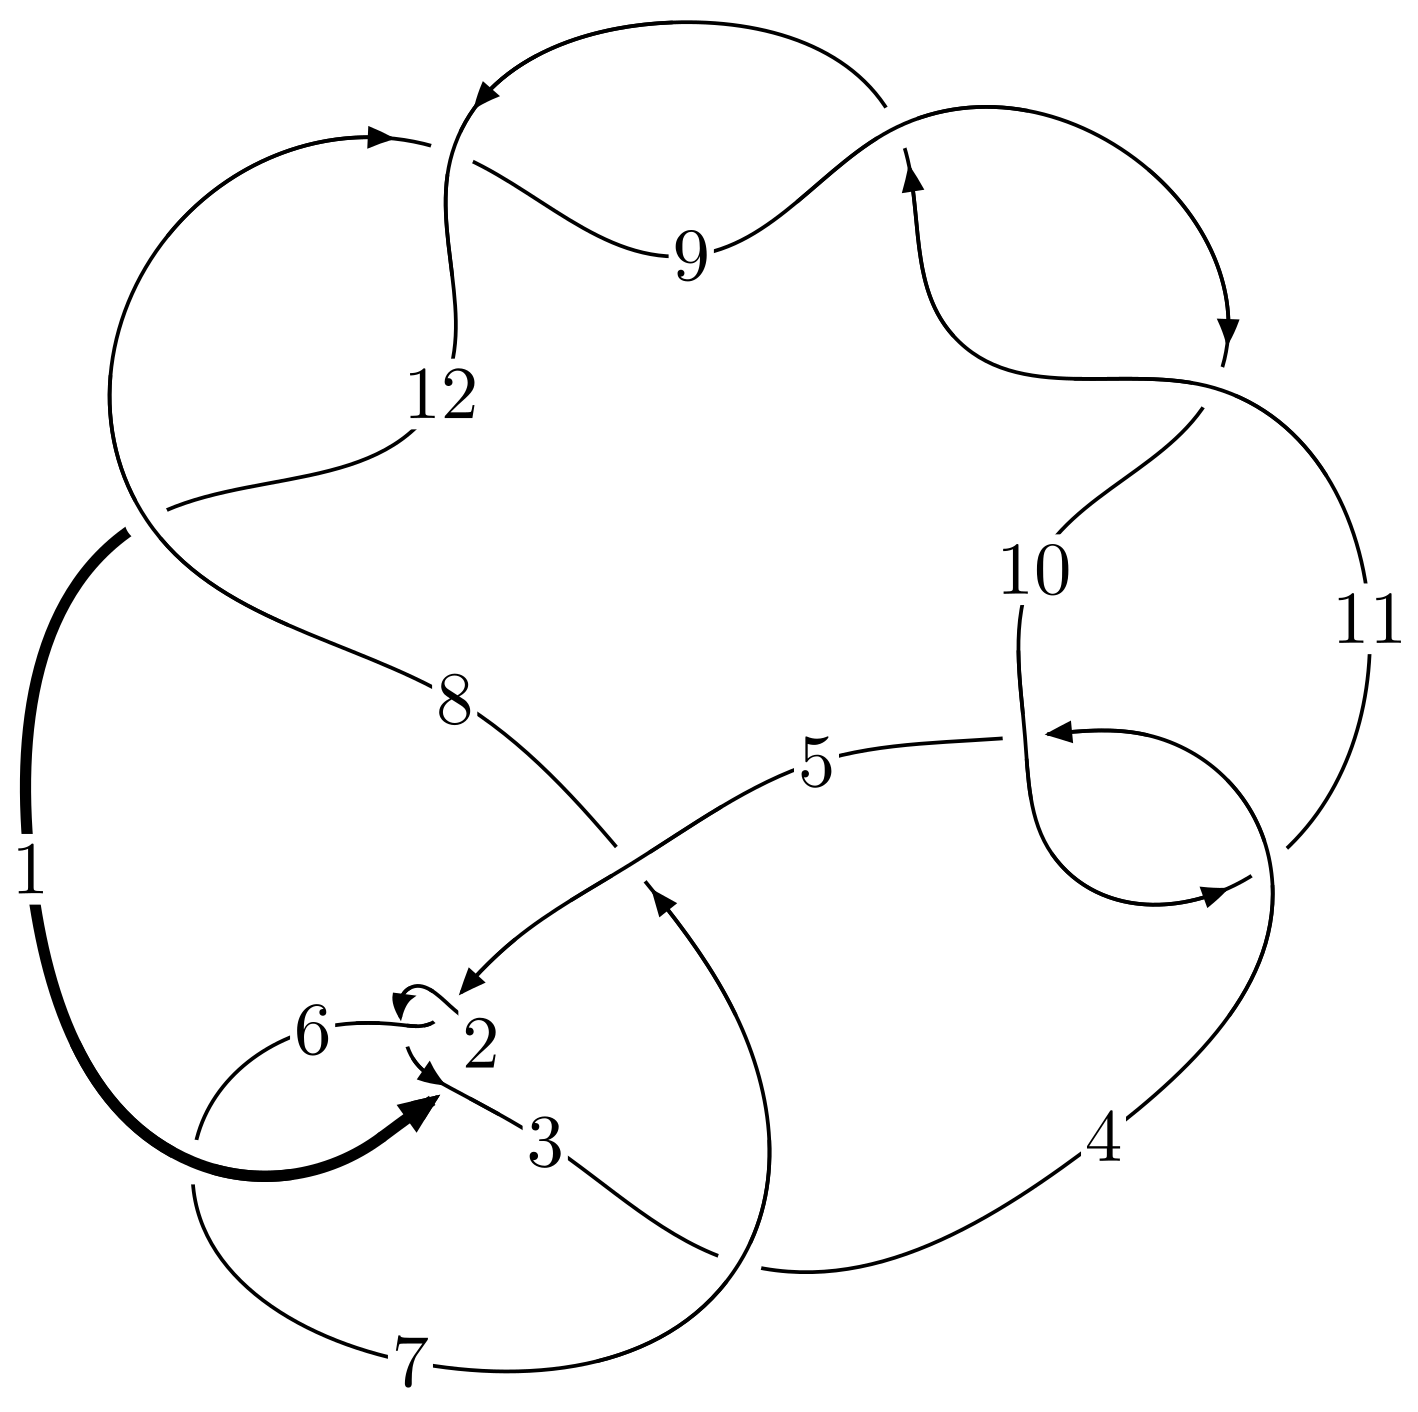
\includegraphics[width=112pt]{../../../GIT/diagram.site/Diagrams/png/1044_12a_0243.png}\\
\ \ \ A knot diagram\footnotemark}&
\allowdisplaybreaks
\textbf{Linearized knot diagam} \\
\cline{2-2}
 &
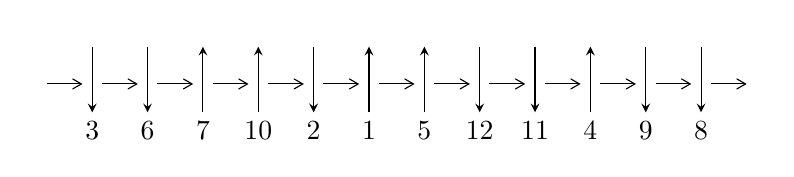
\begin{tikzpicture}[x=20pt, y=17pt]
	% nodes
	\node (C0) at (0, 0) {};
	\node (C1) at (1, 0) {};
	\node (C1U) at (1, +1) {};
	\node (C1D) at (1, -1) {3};

	\node (C2) at (2, 0) {};
	\node (C2U) at (2, +1) {};
	\node (C2D) at (2, -1) {6};

	\node (C3) at (3, 0) {};
	\node (C3U) at (3, +1) {};
	\node (C3D) at (3, -1) {7};

	\node (C4) at (4, 0) {};
	\node (C4U) at (4, +1) {};
	\node (C4D) at (4, -1) {10};

	\node (C5) at (5, 0) {};
	\node (C5U) at (5, +1) {};
	\node (C5D) at (5, -1) {2};

	\node (C6) at (6, 0) {};
	\node (C6U) at (6, +1) {};
	\node (C6D) at (6, -1) {1};

	\node (C7) at (7, 0) {};
	\node (C7U) at (7, +1) {};
	\node (C7D) at (7, -1) {5};

	\node (C8) at (8, 0) {};
	\node (C8U) at (8, +1) {};
	\node (C8D) at (8, -1) {12};

	\node (C9) at (9, 0) {};
	\node (C9U) at (9, +1) {};
	\node (C9D) at (9, -1) {11};

	\node (C10) at (10, 0) {};
	\node (C10U) at (10, +1) {};
	\node (C10D) at (10, -1) {4};

	\node (C11) at (11, 0) {};
	\node (C11U) at (11, +1) {};
	\node (C11D) at (11, -1) {9};

	\node (C12) at (12, 0) {};
	\node (C12U) at (12, +1) {};
	\node (C12D) at (12, -1) {8};
	\node (C13) at (13, 0) {};

	% arrows
	\draw[->,>={angle 60}]
	(C0) edge (C1) (C1) edge (C2) (C2) edge (C3) (C3) edge (C4) (C4) edge (C5) (C5) edge (C6) (C6) edge (C7) (C7) edge (C8) (C8) edge (C9) (C9) edge (C10) (C10) edge (C11) (C11) edge (C12) (C12) edge (C13) ;	\draw[->,>=stealth]
	(C1U) edge (C1D) (C2U) edge (C2D) (C3D) edge (C3U) (C4D) edge (C4U) (C5U) edge (C5D) (C6D) edge (C6U) (C7D) edge (C7U) (C8U) edge (C8D) (C9U) edge (C9D) (C10D) edge (C10U) (C11U) edge (C11D) (C12U) edge (C12D) ;
	\end{tikzpicture} \\
\hhline{~~} \\& 
\textbf{Solving Sequence} \\ \cline{2-2} 
 &
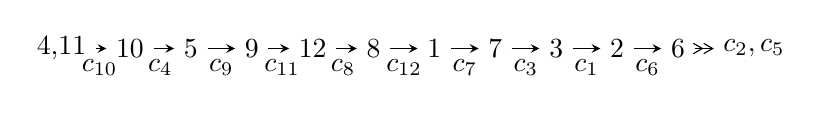
\begin{tikzpicture}[x=22pt, y=7pt]
	% node
	\node (A0) at (-1/8, 0) {4,11};
	\node (A1) at (1, 0) {10};
	\node (A2) at (2, 0) {5};
	\node (A3) at (3, 0) {9};
	\node (A4) at (4, 0) {12};
	\node (A5) at (5, 0) {8};
	\node (A6) at (6, 0) {1};
	\node (A7) at (7, 0) {7};
	\node (A8) at (8, 0) {3};
	\node (A9) at (9, 0) {2};
	\node (A10) at (10, 0) {6};
	\node (C1) at (1/2, -1) {$c_{10}$};
	\node (C2) at (3/2, -1) {$c_{4}$};
	\node (C3) at (5/2, -1) {$c_{9}$};
	\node (C4) at (7/2, -1) {$c_{11}$};
	\node (C5) at (9/2, -1) {$c_{8}$};
	\node (C6) at (11/2, -1) {$c_{12}$};
	\node (C7) at (13/2, -1) {$c_{7}$};
	\node (C8) at (15/2, -1) {$c_{3}$};
	\node (C9) at (17/2, -1) {$c_{1}$};
	\node (C10) at (19/2, -1) {$c_{6}$};
	\node (A11) at (45/4, 0) {$c_{2},c_{5}$};

	% edge
	\draw[->,>=stealth]	
	(A0) edge (A1) (A1) edge (A2) (A2) edge (A3) (A3) edge (A4) (A4) edge (A5) (A5) edge (A6) (A6) edge (A7) (A7) edge (A8) (A8) edge (A9) (A9) edge (A10) ;
	\draw[->>,>={angle 60}]	
	(A10) edge (A11);
\end{tikzpicture} \\ 

\end{tabular} \\

\footnotetext{
The image of knot diagram is generated by the software ``\textbf{Draw programme}" developed by Andrew Bartholomew(\url{http://www.layer8.co.uk/maths/draw/index.htm\#Running-draw}), where we modified some parts for our purpose(\url{https://github.com/CATsTAILs/LinksPainter}).
}\phantom \\ \newline 
\centering \textbf{Ideals for irreducible components\footnotemark of $X_{\text{par}}$} 
 
\begin{align*}
I^u_{1}&=\langle 
u^{66}+u^{65}+\cdots+u+1\rangle \\
\\
\end{align*}
\raggedright * 1 irreducible components of $\dim_{\mathbb{C}}=0$, with total 66 representations.\\
\footnotetext{All coefficients of polynomials are rational numbers. But the coefficients are sometimes approximated in decimal forms when there is not enough margin.}
\newpage
\renewcommand{\arraystretch}{1}
\centering \section*{I. $I^u_{1}= \langle u^{66}+u^{65}+\cdots+u+1 \rangle$}
\flushleft \textbf{(i) Arc colorings}\\
\begin{tabular}{m{7pt} m{180pt} m{7pt} m{180pt} }
\flushright $a_{4}=$&$\begin{pmatrix}0\\u\end{pmatrix}$ \\
\flushright $a_{11}=$&$\begin{pmatrix}1\\0\end{pmatrix}$ \\
\flushright $a_{10}=$&$\begin{pmatrix}1\\u^2\end{pmatrix}$ \\
\flushright $a_{5}=$&$\begin{pmatrix}u\\u^3+u\end{pmatrix}$ \\
\flushright $a_{9}=$&$\begin{pmatrix}u^2+1\\u^2\end{pmatrix}$ \\
\flushright $a_{12}=$&$\begin{pmatrix}u^4+u^2+1\\u^4\end{pmatrix}$ \\
\flushright $a_{8}=$&$\begin{pmatrix}u^6+u^4+2 u^2+1\\u^6+u^2\end{pmatrix}$ \\
\flushright $a_{1}=$&$\begin{pmatrix}u^8+u^6+3 u^4+2 u^2+1\\u^8+2 u^4\end{pmatrix}$ \\
\flushright $a_{7}=$&$\begin{pmatrix}u^{10}+u^8+4 u^6+3 u^4+3 u^2+1\\u^{12}+2 u^{10}+4 u^8+6 u^6+3 u^4+2 u^2\end{pmatrix}$ \\
\flushright $a_{3}=$&$\begin{pmatrix}- u^{21}-2 u^{19}+\cdots-6 u^3- u\\- u^{23}-3 u^{21}+\cdots-2 u^3+u\end{pmatrix}$ \\
\flushright $a_{2}=$&$\begin{pmatrix}u^{52}+5 u^{50}+\cdots+u^2+1\\u^{54}+6 u^{52}+\cdots-17 u^6+u^2\end{pmatrix}$ \\
\flushright $a_{6}=$&$\begin{pmatrix}- u^{28}-3 u^{26}+\cdots+u^2+1\\- u^{28}-2 u^{26}+\cdots+3 u^4+2 u^2\end{pmatrix}$\\&\end{tabular}
\flushleft \textbf{(ii) Obstruction class $= -1$}\\~\\
\flushleft \textbf{(iii) Cusp Shapes $= -4 u^{64}-4 u^{63}+\cdots-4 u-6$}\\~\\
\newpage\renewcommand{\arraystretch}{1}
\flushleft \textbf{(iv) u-Polynomials at the component}\newline \\
\begin{tabular}{m{50pt}|m{274pt}}
Crossings & \hspace{64pt}u-Polynomials at each crossing \\
\hline $$\begin{aligned}c_{1}\end{aligned}$$&$\begin{aligned}
&u^{66}+31 u^{65}+\cdots- u+1
\end{aligned}$\\
\hline $$\begin{aligned}c_{2},c_{5}\end{aligned}$$&$\begin{aligned}
&u^{66}+u^{65}+\cdots+3 u+1
\end{aligned}$\\
\hline $$\begin{aligned}c_{3}\end{aligned}$$&$\begin{aligned}
&u^{66}- u^{65}+\cdots+1669 u+673
\end{aligned}$\\
\hline $$\begin{aligned}c_{4},c_{10}\end{aligned}$$&$\begin{aligned}
&u^{66}+u^{65}+\cdots+u+1
\end{aligned}$\\
\hline $$\begin{aligned}c_{6}\end{aligned}$$&$\begin{aligned}
&u^{66}+3 u^{65}+\cdots+539 u+105
\end{aligned}$\\
\hline $$\begin{aligned}c_{7}\end{aligned}$$&$\begin{aligned}
&u^{66}+9 u^{65}+\cdots+113 u+29
\end{aligned}$\\
\hline $$\begin{aligned}c_{8},c_{9},c_{11}\\c_{12}\end{aligned}$$&$\begin{aligned}
&u^{66}+13 u^{65}+\cdots+u+1
\end{aligned}$\\
\hline
\end{tabular}\\~\\
\newpage\renewcommand{\arraystretch}{1}
\flushleft \textbf{(v) Riley Polynomials at the component}\newline \\
\begin{tabular}{m{50pt}|m{274pt}}
Crossings & \hspace{64pt}Riley Polynomials at each crossing \\
\hline $$\begin{aligned}c_{1}\end{aligned}$$&$\begin{aligned}
&y^{66}+9 y^{65}+\cdots+9 y+1
\end{aligned}$\\
\hline $$\begin{aligned}c_{2},c_{5}\end{aligned}$$&$\begin{aligned}
&y^{66}-31 y^{65}+\cdots+y+1
\end{aligned}$\\
\hline $$\begin{aligned}c_{3}\end{aligned}$$&$\begin{aligned}
&y^{66}-23 y^{65}+\cdots-12012391 y+452929
\end{aligned}$\\
\hline $$\begin{aligned}c_{4},c_{10}\end{aligned}$$&$\begin{aligned}
&y^{66}+13 y^{65}+\cdots+y+1
\end{aligned}$\\
\hline $$\begin{aligned}c_{6}\end{aligned}$$&$\begin{aligned}
&y^{66}+13 y^{65}+\cdots+356909 y+11025
\end{aligned}$\\
\hline $$\begin{aligned}c_{7}\end{aligned}$$&$\begin{aligned}
&y^{66}-11 y^{65}+\cdots+23481 y+841
\end{aligned}$\\
\hline $$\begin{aligned}c_{8},c_{9},c_{11}\\c_{12}\end{aligned}$$&$\begin{aligned}
&y^{66}+81 y^{65}+\cdots-7 y+1
\end{aligned}$\\
\hline
\end{tabular}\\~\\
\newpage\flushleft \textbf{(vi) Complex Volumes and Cusp Shapes}
$$\begin{array}{c|c|c}  
\text{Solutions to }I^u_{1}& \I (\text{vol} + \sqrt{-1}CS) & \text{Cusp shape}\\
 \hline 
\begin{aligned}
u &= \phantom{-}0.599044 + 0.826443 I\end{aligned}
 & \phantom{-}2.20023 + 0.03981 I & \phantom{-}1.90801 + 0. I\phantom{ +0.000000I} \\ \hline\begin{aligned}
u &= \phantom{-}0.599044 - 0.826443 I\end{aligned}
 & \phantom{-}2.20023 - 0.03981 I & \phantom{-}1.90801 + 0. I\phantom{ +0.000000I} \\ \hline\begin{aligned}
u &= \phantom{-}0.516168 + 0.894544 I\end{aligned}
 & -2.24111 + 4.14051 I & -5.37917 - 5.76586 I \\ \hline\begin{aligned}
u &= \phantom{-}0.516168 - 0.894544 I\end{aligned}
 & -2.24111 - 4.14051 I & -5.37917 + 5.76586 I \\ \hline\begin{aligned}
u &= -0.575209 + 0.860059 I\end{aligned}
 & \phantom{-}3.33392 - 4.67344 I & \phantom{-}3.60111 + 7.51773 I \\ \hline\begin{aligned}
u &= -0.575209 - 0.860059 I\end{aligned}
 & \phantom{-}3.33392 + 4.67344 I & \phantom{-}3.60111 - 7.51773 I \\ \hline\begin{aligned}
u &= -0.417668 + 0.858179 I\end{aligned}
 & -3.47104 - 4.65742 I & -7.34835 + 7.77657 I \\ \hline\begin{aligned}
u &= -0.417668 - 0.858179 I\end{aligned}
 & -3.47104 + 4.65742 I & -7.34835 - 7.77657 I \\ \hline\begin{aligned}
u &= -0.548997 + 0.901918 I\end{aligned}
 & \phantom{-}2.20323 - 6.68220 I & \phantom{-0.000000 -}0. + 7.34850 I \\ \hline\begin{aligned}
u &= -0.548997 - 0.901918 I\end{aligned}
 & \phantom{-}2.20323 + 6.68220 I & \phantom{-0.000000 } 0. - 7.34850 I \\ \hline\begin{aligned}
u &= \phantom{-}0.662569 + 0.668001 I\end{aligned}
 & \phantom{-}2.71906 + 4.65572 I & \phantom{-}3.37494 - 5.91636 I \\ \hline\begin{aligned}
u &= \phantom{-}0.662569 - 0.668001 I\end{aligned}
 & \phantom{-}2.71906 - 4.65572 I & \phantom{-}3.37494 + 5.91636 I \\ \hline\begin{aligned}
u &= \phantom{-}0.545262 + 0.916750 I\end{aligned}
 & -0.02627 + 11.64450 I & \phantom{-0.000000 } 0. - 11.11786 I \\ \hline\begin{aligned}
u &= \phantom{-}0.545262 - 0.916750 I\end{aligned}
 & -0.02627 - 11.64450 I & \phantom{-0.000000 -}0. + 11.11786 I \\ \hline\begin{aligned}
u &= -0.658358 + 0.624266 I\end{aligned}
 & \phantom{-}4.09825 + 0.06503 I & \phantom{-}6.21402 - 0.17680 I \\ \hline\begin{aligned}
u &= -0.658358 - 0.624266 I\end{aligned}
 & \phantom{-}4.09825 - 0.06503 I & \phantom{-}6.21402 + 0.17680 I \\ \hline\begin{aligned}
u &= -0.331173 + 0.844557 I\end{aligned}
 & -2.52809 + 2.55717 I & -6.16177 + 0.11362 I \\ \hline\begin{aligned}
u &= -0.331173 - 0.844557 I\end{aligned}
 & -2.52809 - 2.55717 I & -6.16177 - 0.11362 I \\ \hline\begin{aligned}
u &= -0.111108 + 0.897806 I\end{aligned}
 & -3.65266 - 7.15580 I & -8.25035 + 7.79317 I \\ \hline\begin{aligned}
u &= -0.111108 - 0.897806 I\end{aligned}
 & -3.65266 + 7.15580 I & -8.25035 - 7.79317 I \\ \hline\begin{aligned}
u &= -0.056026 + 0.881651 I\end{aligned}
 & -5.32447 + 0.22926 I & -11.87724 + 0.46623 I \\ \hline\begin{aligned}
u &= -0.056026 - 0.881651 I\end{aligned}
 & -5.32447 - 0.22926 I & -11.87724 - 0.46623 I \\ \hline\begin{aligned}
u &= \phantom{-}0.112571 + 0.866237 I\end{aligned}
 & -1.39262 + 2.45864 I & -5.10441 - 4.27623 I \\ \hline\begin{aligned}
u &= \phantom{-}0.112571 - 0.866237 I\end{aligned}
 & -1.39262 - 2.45864 I & -5.10441 + 4.27623 I \\ \hline\begin{aligned}
u &= -0.669205 + 0.554761 I\end{aligned}
 & \phantom{-}3.32166 + 2.13457 I & \phantom{-}5.05558 - 0.87891 I \\ \hline\begin{aligned}
u &= -0.669205 - 0.554761 I\end{aligned}
 & \phantom{-}3.32166 - 2.13457 I & \phantom{-}5.05558 + 0.87891 I \\ \hline\begin{aligned}
u &= \phantom{-}0.683206 + 0.533126 I\end{aligned}
 & \phantom{-}1.20996 - 7.07293 I & \phantom{-}1.66097 + 5.05839 I \\ \hline\begin{aligned}
u &= \phantom{-}0.683206 - 0.533126 I\end{aligned}
 & \phantom{-}1.20996 + 7.07293 I & \phantom{-}1.66097 - 5.05839 I \\ \hline\begin{aligned}
u &= \phantom{-}0.397569 + 0.766288 I\end{aligned}
 & -0.23774 + 1.55359 I & -1.92023 - 4.37944 I \\ \hline\begin{aligned}
u &= \phantom{-}0.397569 - 0.766288 I\end{aligned}
 & -0.23774 - 1.55359 I & -1.92023 + 4.37944 I\\
 \hline 
 \end{array}$$\newpage$$\begin{array}{c|c|c}  
\text{Solutions to }I^u_{1}& \I (\text{vol} + \sqrt{-1}CS) & \text{Cusp shape}\\
 \hline 
\begin{aligned}
u &= \phantom{-}0.610588 + 0.515135 I\end{aligned}
 & -1.056340 + 0.121936 I & -1.71551 - 0.70249 I \\ \hline\begin{aligned}
u &= \phantom{-}0.610588 - 0.515135 I\end{aligned}
 & -1.056340 - 0.121936 I & -1.71551 + 0.70249 I \\ \hline\begin{aligned}
u &= \phantom{-}0.188820 + 0.739972 I\end{aligned}
 & -0.49246 + 1.40224 I & -3.25312 - 5.95695 I \\ \hline\begin{aligned}
u &= \phantom{-}0.188820 - 0.739972 I\end{aligned}
 & -0.49246 - 1.40224 I & -3.25312 + 5.95695 I \\ \hline\begin{aligned}
u &= \phantom{-}0.868041 + 0.906909 I\end{aligned}
 & \phantom{-}4.33013 - 0.66559 I & \phantom{-0.000000 } 0 \\ \hline\begin{aligned}
u &= \phantom{-}0.868041 - 0.906909 I\end{aligned}
 & \phantom{-}4.33013 + 0.66559 I & \phantom{-0.000000 } 0 \\ \hline\begin{aligned}
u &= \phantom{-}0.860634 + 0.928908 I\end{aligned}
 & \phantom{-}4.26183 + 7.07643 I & \phantom{-0.000000 } 0 \\ \hline\begin{aligned}
u &= \phantom{-}0.860634 - 0.928908 I\end{aligned}
 & \phantom{-}4.26183 - 7.07643 I & \phantom{-0.000000 } 0 \\ \hline\begin{aligned}
u &= -0.873798 + 0.921550 I\end{aligned}
 & \phantom{-}7.45184 - 3.23504 I & \phantom{-0.000000 } 0 \\ \hline\begin{aligned}
u &= -0.873798 - 0.921550 I\end{aligned}
 & \phantom{-}7.45184 + 3.23504 I & \phantom{-0.000000 } 0 \\ \hline\begin{aligned}
u &= -0.906361 + 0.896191 I\end{aligned}
 & \phantom{-}6.91112 + 0.26195 I & \phantom{-0.000000 } 0 \\ \hline\begin{aligned}
u &= -0.906361 - 0.896191 I\end{aligned}
 & \phantom{-}6.91112 - 0.26195 I & \phantom{-0.000000 } 0 \\ \hline\begin{aligned}
u &= -0.918035 + 0.894590 I\end{aligned}
 & \phantom{-}9.54527 + 7.87292 I & \phantom{-0.000000 } 0 \\ \hline\begin{aligned}
u &= -0.918035 - 0.894590 I\end{aligned}
 & \phantom{-}9.54527 - 7.87292 I & \phantom{-0.000000 } 0 \\ \hline\begin{aligned}
u &= \phantom{-}0.916098 + 0.898640 I\end{aligned}
 & \phantom{-}11.73460 - 2.74151 I & \phantom{-0.000000 } 0 \\ \hline\begin{aligned}
u &= \phantom{-}0.916098 - 0.898640 I\end{aligned}
 & \phantom{-}11.73460 + 2.74151 I & \phantom{-0.000000 } 0 \\ \hline\begin{aligned}
u &= \phantom{-}0.913249 + 0.910862 I\end{aligned}
 & \phantom{-}12.86730 - 0.20173 I & \phantom{-0.000000 } 0 \\ \hline\begin{aligned}
u &= \phantom{-}0.913249 - 0.910862 I\end{aligned}
 & \phantom{-}12.86730 + 0.20173 I & \phantom{-0.000000 } 0 \\ \hline\begin{aligned}
u &= -0.911288 + 0.917800 I\end{aligned}
 & \phantom{-}11.72190 - 4.80348 I & \phantom{-0.000000 } 0 \\ \hline\begin{aligned}
u &= -0.911288 - 0.917800 I\end{aligned}
 & \phantom{-}11.72190 + 4.80348 I & \phantom{-0.000000 } 0 \\ \hline\begin{aligned}
u &= -0.876349 + 0.959209 I\end{aligned}
 & \phantom{-}6.70835 - 6.84097 I & \phantom{-0.000000 } 0 \\ \hline\begin{aligned}
u &= -0.876349 - 0.959209 I\end{aligned}
 & \phantom{-}6.70835 + 6.84097 I & \phantom{-0.000000 } 0 \\ \hline\begin{aligned}
u &= -0.894477 + 0.950445 I\end{aligned}
 & \phantom{-}11.61560 - 1.85123 I & \phantom{-0.000000 } 0 \\ \hline\begin{aligned}
u &= -0.894477 - 0.950445 I\end{aligned}
 & \phantom{-}11.61560 + 1.85123 I & \phantom{-0.000000 } 0 \\ \hline\begin{aligned}
u &= \phantom{-}0.890410 + 0.955883 I\end{aligned}
 & \phantom{-}12.7211 + 6.8493 I & \phantom{-0.000000 } 0 \\ \hline\begin{aligned}
u &= \phantom{-}0.890410 - 0.955883 I\end{aligned}
 & \phantom{-}12.7211 - 6.8493 I & \phantom{-0.000000 } 0 \\ \hline\begin{aligned}
u &= \phantom{-}0.883095 + 0.964486 I\end{aligned}
 & \phantom{-}11.5212 + 9.3733 I & \phantom{-0.000000 } 0 \\ \hline\begin{aligned}
u &= \phantom{-}0.883095 - 0.964486 I\end{aligned}
 & \phantom{-}11.5212 - 9.3733 I & \phantom{-0.000000 } 0 \\ \hline\begin{aligned}
u &= -0.881274 + 0.967913 I\end{aligned}
 & \phantom{-}9.3076 - 14.5044 I & \phantom{-0.000000 } 0 \\ \hline\begin{aligned}
u &= -0.881274 - 0.967913 I\end{aligned}
 & \phantom{-}9.3076 + 14.5044 I & \phantom{-0.000000 } 0\\
 \hline 
 \end{array}$$\newpage$$\begin{array}{c|c|c}  
\text{Solutions to }I^u_{1}& \I (\text{vol} + \sqrt{-1}CS) & \text{Cusp shape}\\
 \hline 
\begin{aligned}
u &= -0.536662 + 0.126308 I\end{aligned}
 & -0.45344 - 5.38731 I & \phantom{-}1.77316 + 5.79640 I \\ \hline\begin{aligned}
u &= -0.536662 - 0.126308 I\end{aligned}
 & -0.45344 + 5.38731 I & \phantom{-}1.77316 - 5.79640 I \\ \hline\begin{aligned}
u &= -0.469047 + 0.278278 I\end{aligned}
 & -1.96507 + 1.34680 I & -1.73694 - 0.71589 I \\ \hline\begin{aligned}
u &= -0.469047 - 0.278278 I\end{aligned}
 & -1.96507 - 1.34680 I & -1.73694 + 0.71589 I \\ \hline\begin{aligned}
u &= \phantom{-}0.487711 + 0.078072 I\end{aligned}
 & \phantom{-}1.49223 + 0.76367 I & \phantom{-}5.93436 - 1.14172 I \\ \hline\begin{aligned}
u &= \phantom{-}0.487711 - 0.078072 I\end{aligned}
 & \phantom{-}1.49223 - 0.76367 I & \phantom{-}5.93436 + 1.14172 I\\
 \hline 
 \end{array}$$\newpage
\newpage\renewcommand{\arraystretch}{1}
\centering \section*{ II. u-Polynomials}
\begin{tabular}{m{50pt}|m{274pt}}
Crossings & \hspace{64pt}u-Polynomials at each crossing \\
\hline $$\begin{aligned}c_{1}\end{aligned}$$&$\begin{aligned}
&u^{66}+31 u^{65}+\cdots- u+1
\end{aligned}$\\
\hline $$\begin{aligned}c_{2},c_{5}\end{aligned}$$&$\begin{aligned}
&u^{66}+u^{65}+\cdots+3 u+1
\end{aligned}$\\
\hline $$\begin{aligned}c_{3}\end{aligned}$$&$\begin{aligned}
&u^{66}- u^{65}+\cdots+1669 u+673
\end{aligned}$\\
\hline $$\begin{aligned}c_{4},c_{10}\end{aligned}$$&$\begin{aligned}
&u^{66}+u^{65}+\cdots+u+1
\end{aligned}$\\
\hline $$\begin{aligned}c_{6}\end{aligned}$$&$\begin{aligned}
&u^{66}+3 u^{65}+\cdots+539 u+105
\end{aligned}$\\
\hline $$\begin{aligned}c_{7}\end{aligned}$$&$\begin{aligned}
&u^{66}+9 u^{65}+\cdots+113 u+29
\end{aligned}$\\
\hline $$\begin{aligned}c_{8},c_{9},c_{11}\\c_{12}\end{aligned}$$&$\begin{aligned}
&u^{66}+13 u^{65}+\cdots+u+1
\end{aligned}$\\
\hline
\end{tabular}\newpage\renewcommand{\arraystretch}{1}
\centering \section*{ III. Riley Polynomials}
\begin{tabular}{m{50pt}|m{274pt}}
Crossings & \hspace{64pt}Riley Polynomials at each crossing \\
\hline $$\begin{aligned}c_{1}\end{aligned}$$&$\begin{aligned}
&y^{66}+9 y^{65}+\cdots+9 y+1
\end{aligned}$\\
\hline $$\begin{aligned}c_{2},c_{5}\end{aligned}$$&$\begin{aligned}
&y^{66}-31 y^{65}+\cdots+y+1
\end{aligned}$\\
\hline $$\begin{aligned}c_{3}\end{aligned}$$&$\begin{aligned}
&y^{66}-23 y^{65}+\cdots-12012391 y+452929
\end{aligned}$\\
\hline $$\begin{aligned}c_{4},c_{10}\end{aligned}$$&$\begin{aligned}
&y^{66}+13 y^{65}+\cdots+y+1
\end{aligned}$\\
\hline $$\begin{aligned}c_{6}\end{aligned}$$&$\begin{aligned}
&y^{66}+13 y^{65}+\cdots+356909 y+11025
\end{aligned}$\\
\hline $$\begin{aligned}c_{7}\end{aligned}$$&$\begin{aligned}
&y^{66}-11 y^{65}+\cdots+23481 y+841
\end{aligned}$\\
\hline $$\begin{aligned}c_{8},c_{9},c_{11}\\c_{12}\end{aligned}$$&$\begin{aligned}
&y^{66}+81 y^{65}+\cdots-7 y+1
\end{aligned}$\\
\hline
\end{tabular}
\vskip 2pc
\end{document}